Dado un tablero de ajedrez donde se ubican caballos, determine si el tablero es completamente alcanzable (todas sus casillas son alcanzables). Una casilla es alcanzable si algún caballo puede llegar a ella en 0 o 1 movimientos. La representación del tablero será un array bidimensional de bool donde solo habrá true en las casillas donde haya un caballo. 
\begin{itemize}
    \item En este caso se devuelve false ya que solo se alcanzan las casillas \( (0,3), (1,1), (2,3),(3,0), (3,2) \).
    \begin{center}
    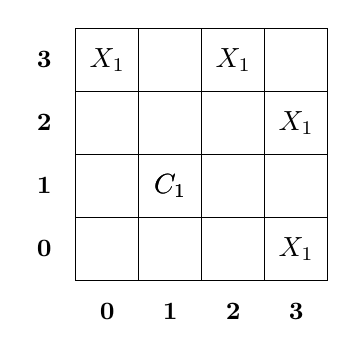
\begin{tikzpicture}[scale=0.8]
        % Dibuja el tablero
        \foreach \x in {0,1,2,3} {
            \foreach \y in {0,1,2,3} {
                \fill[white] (\x,\y) rectangle (\x+1,\y+1);
                \draw (\x,\y) rectangle (\x+1,\y+1);
            }
        }
    
        % Marcar los caballos con C_i
        \node at (1.5, 1.5) {$C_1$}; % (1,1)
    
        % Marcar las casillas alcanzables con X_i
        \node at (0.5, 3.5) {$X_1$}; % (0,3)
        \node at (1.5, 1.5) {$C_1$}; % (1,1)
        \node at (2.5, 3.5) {$X_1$}; % (2,3)
        \node at (3.5, 0.5) {$X_1$}; % (3,0)
        \node at (3.5, 2.5) {$X_1$}; % (3,2)
    
        % Etiquetas
        \foreach \x in {0,...,3} {
            \foreach \y in {0,...,3} {
                % Etiquetas de fila y columna
                \ifnum\x=0
                    \node at (-0.5,\y+0.5) {\textbf{\small \y}};
                \fi
                \ifnum\y=0
                    \node at (\x+0.5,-0.5) {\textbf{\small \x}};
                \fi
            }
        }
    \end{tikzpicture}
    \end{center}
    \item En otro caso se devuelve true pues todas las casillas son alcanzables (algunas por más de un caballo).
    \begin{center}
    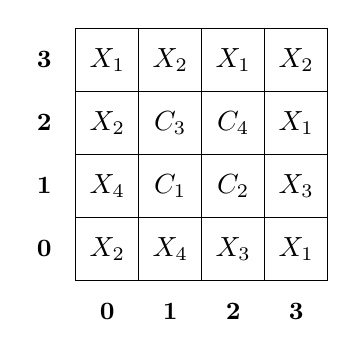
\begin{tikzpicture}[scale=0.8]
        % Dibuja el tablero
        \foreach \x in {0,1,2,3} {
            \foreach \y in {0,1,2,3} {
                \fill[white] (\x,\y) rectangle (\x+1,\y+1);
                \draw (\x,\y) rectangle (\x+1,\y+1);
            }
        }
        
        % Caballos en posiciones C_i
        \node at (1.5, 1.5) {$C_1$}; % (1,1)
        \node at (2.5, 1.5) {$C_2$}; % (2,1)
        \node at (1.5, 2.5) {$C_3$}; % (1,2)
        \node at (2.5, 2.5) {$C_4$}; % (2,2)
    
        % Marcar las casillas alcanzables con X_i
        \node at (0.5, 0.5) {$X_2$}; % (0,0)
        \node at (0.5, 1.5) {$X_4$}; % (0,1)
        \node at (0.5, 2.5) {$X_2$}; % (0,2)
        \node at (0.5, 3.5) {$X_1$}; % (0,3)
        \node at (1.5, 0.5) {$X_4$}; % (1,0)
        \node at (1.5, 3.5) {$X_2$}; % (1,3)
        \node at (2.5, 0.5) {$X_3$}; % (2,0)
        \node at (2.5, 3.5) {$X_1$}; % (2,3)
        \node at (3.5, 0.5) {$X_1$}; % (3,0)
        \node at (3.5, 1.5) {$X_3$}; % (3,1)
        \node at (3.5, 2.5) {$X_1$}; % (3,2)
        \node at (3.5, 3.5) {$X_2$}; % (3,3)
    
        % Etiquetas
        \foreach \x in {0,...,3} {
            \foreach \y in {0,...,3} {
                % Etiquetas de fila y columna
                \ifnum\x=0
                    \node at (-0.5,\y+0.5) {\textbf{\small \y}};
                \fi
                \ifnum\y=0
                    \node at (\x+0.5,-0.5) {\textbf{\small \x}};
                \fi
            }
        }
        
    \end{tikzpicture}
    \end{center}
\end{itemize}